\chapter{ऊष्मागतिकी का पहला नियम}\label{ch:b1:first-law}

साइकिल का टायर फुलाइए और पंप की नली इतनी गरम हो जाती है कि हाथ में पकड़ी
न जाए। डीज़ल इंजन में कोई स्फुलिंग-प्लग नहीं होता: वह अपनी हवा को बीस गुना
छोटा दबा देता है, और हवा इतनी गरम हो जाती है कि ईंधन अपने आप जल उठे।
संपीडित गैस का कोई सिलेंडर खाली होते-होते अपने ऊपर पाला जमा लेता है। हर
बार ऊर्जा रूप बदलती है --- कार्य \omterm{def:b1:first-law:heat}{ऊष्मा} बनता है, \omterm{def:b1:first-law:heat}{ऊष्मा} कार्य, और दोनों
\omterm{def:b1:kinetic-theory:U}{आंतरिक ऊर्जा} --- और \omterm{thm:b1:first-law:firstlaw}{ऊष्मागतिकी का पहला नियम} वही बहीखाता है जो हिसाब बराबर
रखता है। यह अध्याय किसी \omterm{def:b1:first-law:transformation}{ऊष्मागतिक निकाय} के लिए कार्य और \omterm{def:b1:first-law:heat}{ऊष्मा} को परिभाषित
करता है, पहला नियम बताता है, \omterm{def:b1:kinetic-theory:U}{आंतरिक ऊर्जा} तथा \omterm{def:b1:first-law:enthalpy}{एन्थैल्पी} को उन राशियों के
रूप में लाता है जिन्हें वह संरक्षित रखता है, और उसे \omterm{def:b1:kinetic-theory:model}{आदर्श गैस} के रूपांतरणों
तथा ऊष्मामिति पर लगाता है।

\begin{omfigure}
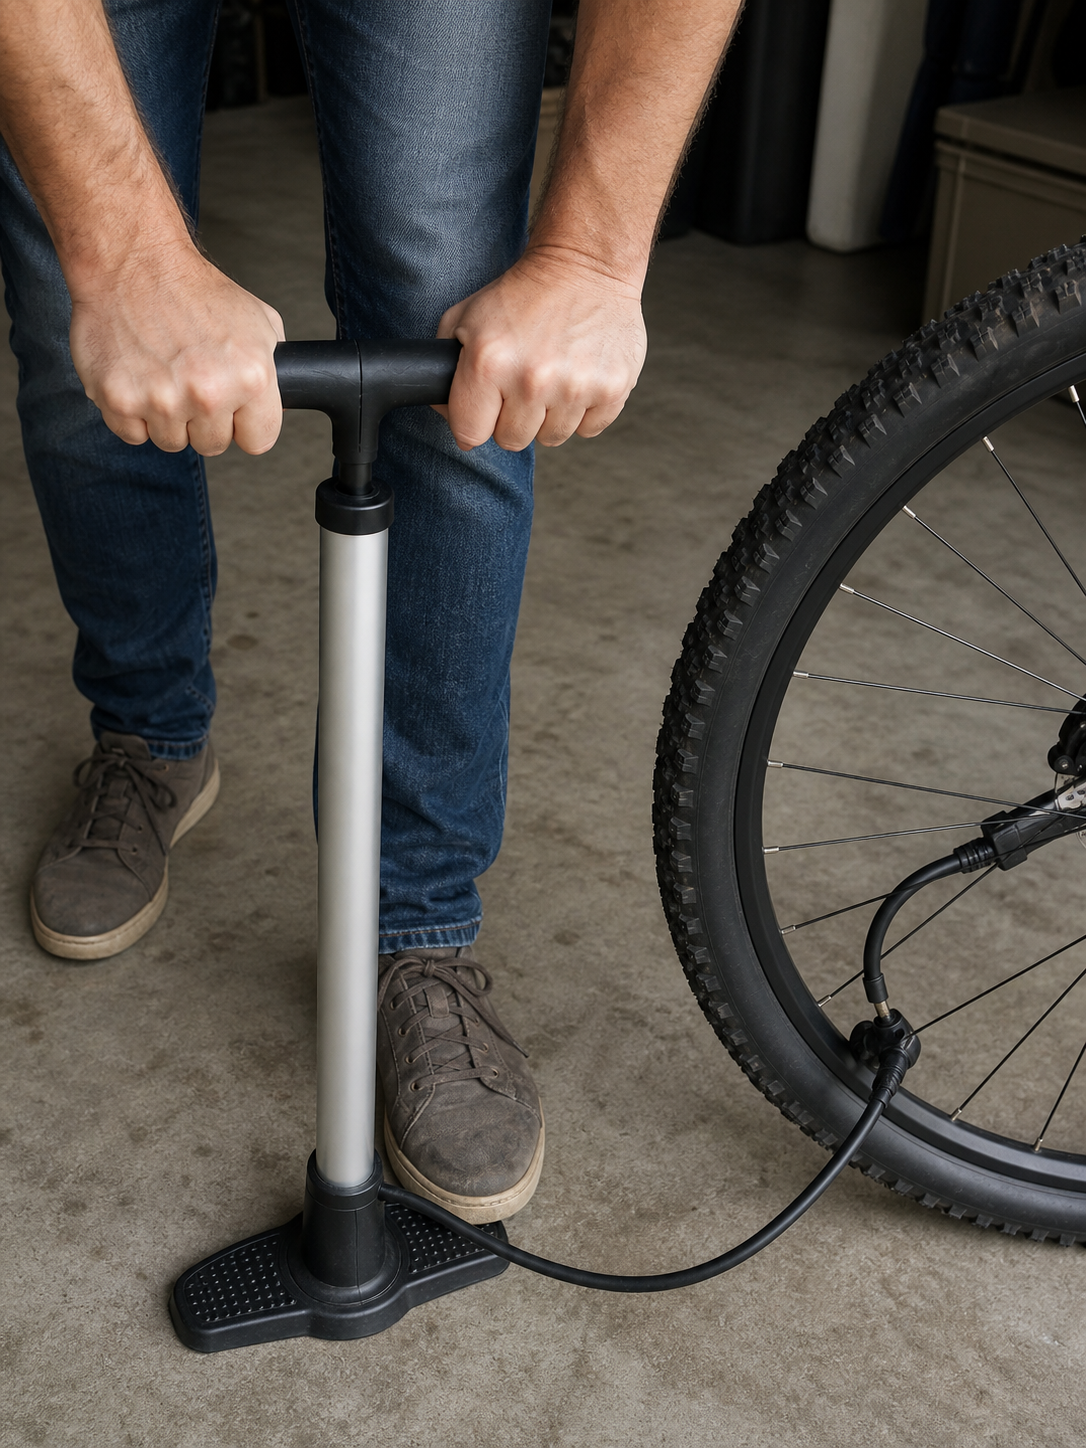
\includegraphics[width=0.36\linewidth]{images/book3/ai/b3-22-bicycle-pump.png}

{\small साइकिल का पंप: फँसी हुई हवा पर हाथ का कार्य उसकी \omterm{def:b1:kinetic-theory:U}{आंतरिक ऊर्जा} बढ़ा देता है, और नली गरम हो जाती है --- यानी हथेली में पहला नियम।}
\end{omfigure}

\section{रूपांतरण, कार्य और ऊष्मा}

\begin{definition}[निकाय, रूपांतरण]\label{def:b1:first-law:transformation}
\index{ऊष्मागतिक निकाय}\index{रूपांतरण}\index{अर्ध-स्थैतिक रूपांतरण}\index{उत्क्रमणीय रूपांतरण}
\emph{ऊष्मागतिक निकाय} किसी चुनी हुई सीमा के भीतर का पदार्थ है; और बाकी सब
\emph{परिवेश}। कोई \emph{रूपांतरण} उसे एक साम्य अवस्था से दूसरी तक ले जाता
है। वह \emph{अर्ध-स्थैतिक} है यदि निकाय साम्य अवस्थाओं की एक शृंखला से
होकर गुज़रे (यानी इतना धीमा कि $P$, $T$ हर जगह परिभाषित रहें), और
\emph{उत्क्रमणीय} यदि, इसके अलावा, बाहरी परिस्थितियाँ उलट देने से पथ भी
उलट जाए (कोई घर्षण नहीं, परिवेश से ताप या दाब का कोई परिमित अंतर नहीं)।
नाम इस पर पड़ते हैं कि क्या अचर रहता है: \emph{समतापी} ($T$),
\emph{समदाबी} ($P$), \emph{समआयतनिक} ($V$); और \emph{रुद्धोष्म} यदि कोई
\omterm{def:b1:first-law:heat}{ऊष्मा} का आदान-प्रदान न हो; \emph{एकदाबी} (\emph{एकतापी}) यदि बाहरी दाब
(ताप) अचर हो, भीतर चाहे कुछ भी होता रहे।
\end{definition}

\begin{proposition}[दाब-बलों का कार्य]\label{prop:b1:first-law:work}
\index{कार्य!दाब-बलों का}
जिस निकाय का आयतन $\dd V$ से बदले, किसी बाहरी दाब $P_{\mathrm{ext}}$ के
विरुद्ध, उसे यह कार्य मिलता है
\[
\delta W = -P_{\mathrm{ext}}\,\dd V, \qquad
W = -\int_{V_1}^{V_2}P_{\mathrm{ext}}\,\dd V .
\]
\omterm{def:b1:first-law:transformation}{अर्ध-स्थैतिक रूपांतरण} के लिए $P_{\mathrm{ext}} = P$ होता है (यानी निकाय का
अपना दाब) और $W = -\int P\,\dd V$ क्लैपेरॉन आरेख में पथ के नीचे का
क्षेत्रफल है, ऋण चिह्न के साथ: संपीडन में धनात्मक, प्रसार में ऋणात्मक।
\end{proposition}

\begin{proof}
$S$ क्षेत्रफल का कोई पिस्टन, जिसे परिवेश बल $P_{\mathrm{ext}}S$ से धकेलता
है, बाहर की ओर $\dd x$ खिसक जाता है: परिवेश निकाय पर
$-P_{\mathrm{ext}}S\,\dd x = -P_{\mathrm{ext}}\,\dd V$ कार्य करता है। कोई भी
सीमा ऐसे ही पिस्टनों का समूह है। अर्ध-स्थैतिक में: पिस्टन साम्य में है, अतः
लुप्त होते अंतर तक $P_{\mathrm{ext}} = P$।
\end{proof}

\begin{definition}[ऊष्मा]\label{def:b1:first-law:heat}
\index{ऊष्मा}\index{ऊष्मा-भंडार}
\emph{ऊष्मा} $Q$ वह ऊर्जा है जो निकाय को स्थूल कार्य के अलावा किसी और ढंग
से मिले --- किसी दीवार पर आणविक टक्करों से (चालन), किसी तरल के परिसंचरण से
(संवहन), या विकिरण से। \emph{ऊष्मा-भंडार} इतना बड़ा पिंड है कि वह जितनी भी
ऊष्मा का आदान-प्रदान करे, उसका ताप नहीं बदलता। पूरे खंड में चिह्न-संकेत
यही है: $W$ और $Q$ निकाय को \emph{मिले} हुए हैं, और भीतर आने पर धनात्मक।
\end{definition}

\section{पहला नियम}

\begin{theorem}[ऊष्मागतिकी का पहला नियम]\label{thm:b1:first-law:firstlaw}
\index{ऊष्मागतिकी का पहला नियम}\index{आंतरिक ऊर्जा}
किसी \omterm{def:b1:newton-dynamics:conservation}{संवृत निकाय} के पास एक अवस्था फलन होता है, उसकी \emph{\omterm{def:b1:kinetic-theory:U}{आंतरिक ऊर्जा}}
$U$ (विस्तीर्ण), जिससे किसी भी \omterm{def:b1:first-law:transformation}{रूपांतरण} के लिए
\[
\Delta U + \Delta E_{k} = W + Q ,
\]
जहाँ $E_k$ स्थूल \omterm{thm:b1:work-and-energy:ke}{गतिज ऊर्जा} है (विराम में पड़े निकाय के लिए शून्य): यानी
कार्य और \omterm{def:b1:first-law:heat}{ऊष्मा} के रूप में मिली ऊर्जा \omterm{def:b1:kinetic-theory:U}{आंतरिक ऊर्जा} के रूप में संचित हो
जाती है। $W$ और $Q$ में से हर एक पथ पर निर्भर करता है; उनका योग नहीं।
\end{theorem}
\admitted

\begin{remark}[यह कहता क्या है]\label{rem:b1:first-law:meaning}
यह ऊर्जा-संरक्षण ही है, जिसमें \omterm{def:b1:first-law:heat}{ऊष्मा} को ऊर्जा के एक हस्तांतरण के रूप में
पहचान लिया गया है (जूल का चक्री-प्रयोग: कोई मापा गया कार्य पानी का ताप
हमेशा उतना ही बढ़ाता है जितनी कोई मापी गई \omterm{def:b1:first-law:heat}{ऊष्मा})। ``$U$ एक अवस्था फलन है''
का अर्थ है कि $\Delta U$ आरंभिक और अंतिम अवस्थाओं से तय हो जाता है ---
अतः किसी चक्र में $\Delta U = 0$ और $W + Q = 0$: यानी जो इंजन कार्य देता
है उसे \omterm{def:b1:first-law:heat}{ऊष्मा} लेनी ही पड़ती है। $U$ की सूक्ष्म अंतर्वस्तु वही है जो
\cref{def:b1:kinetic-theory:U} में है।
\end{remark}

\begin{definition}[एन्थैल्पी; ऊष्मा धारिताएँ]\label{def:b1:first-law:enthalpy}
\index{एन्थैल्पी}\index{स्थिर दाब पर ऊष्मा धारिता}
\emph{एन्थैल्पी} $H = U + PV$ एक अवस्था फलन है, जो अचर दाब पर होते
रूपांतरणों के लिए उपयुक्त है। \emph{स्थिर आयतन और स्थिर दाब पर \omterm{def:b1:first-law:heat}{ऊष्मा}
धारिताएँ} ये हैं
\[
C_V = \left(\frac{\partial U}{\partial T}\right)_V, \qquad
C_P = \left(\frac{\partial H}{\partial T}\right)_P ,
\]
जो \unit{J/K} में हैं; प्रति \omterm{def:b1:kinetic-theory:scales}{मोल} $C_{V,m}$, $C_{P,m}$; और प्रति किलोग्राम
विशिष्ट ऊष्माएँ $c_V$, $c_P$।
\end{definition}

\begin{proposition}[स्थिर आयतन पर और स्थिर दाब पर ऊष्मा]\label{prop:b1:first-law:qvqp}
विराम में पड़े ऐसे निकाय के लिए जो कार्य का आदान-प्रदान केवल दाब-बलों से करे:
\begin{itemize}
  \item समआयतनिक \omterm{def:b1:first-law:transformation}{रूपांतरण}: $W = 0$ और $Q_V = \Delta U$;
  \item बाहरी दाब $P_0$ पर की दो अवस्थाओं के बीच एकदाबी \omterm{def:b1:first-law:transformation}{रूपांतरण}:
        $Q_P = \Delta H$।
\end{itemize}
\end{proposition}

\begin{proof}
समआयतनिक: $\dd V = 0$। एकदाबी: $W = -P_0(V_2 - V_1)$, अतः $Q = \Delta U +
P_0\Delta V = \Delta(U + PV)$, क्योंकि $P_1 = P_2 = P_0$।
\end{proof}

\begin{proposition}[आदर्श गैस: $U$, $H$, मेयर का संबंध]\label{prop:b1:first-law:gas}
\index{मेयर का संबंध}\index{रुद्धोष्म चरघातांक}\index{जूल के नियम}
\omterm{def:b1:kinetic-theory:model}{आदर्श गैस} के लिए $U$ और $H$ केवल $T$ पर निर्भर करते हैं (\omterm{prop:b1:kinetic-theory:Ugas}{जूल के नियम}):
$\dd U = C_V\,\dd T$, $\dd H = C_P\,\dd T$, और
\[
C_{P,m} - C_{V,m} = R, \qquad \gamma = \frac{C_P}{C_V}, \qquad
C_{V,m} = \frac{R}{\gamma - 1}, \quad C_{P,m} = \frac{\gamma R}{\gamma - 1} ;
\]
एकपरमाणुक गैसों के लिए $\gamma = 5/3$, और साधारण तापों पर द्विपरमाणुक
गैसों के लिए $7/5$। \cref{prop:b1:kinetic-theory:condensed} के प्रतिरूप में
किसी \omterm{prop:b1:kinetic-theory:condensed}{संघनित प्रावस्था} के लिए, $C_P \approx C_V = C$ और
$\dd U \approx \dd H = C\,\dd T$।
\end{proposition}

\begin{proof}
$H = U + nRT$; इसे $T$ के सापेक्ष अवकलित कीजिए।
\cref{prop:b1:kinetic-theory:Ugas} से $C_{V,m} = \tfrac32 R$ या $\tfrac52 R$।
\end{proof}

\section{आदर्श गैस के रूपांतरण}

\begin{proposition}[चार मानक रूपांतरण]\label{prop:b1:first-law:transformations}
\index{समतापी रूपांतरण}\index{रुद्धोष्म रूपांतरण}\index{लाप्लास का नियम}
\omterm{def:b1:kinetic-theory:model}{आदर्श गैस} के $n$ मोलों के लिए:
\begin{itemize}
  \item समआयतनिक: $W = 0$, $Q = \Delta U = nC_{V,m}\Delta T$;
  \item समदाबी (अर्ध-स्थैतिक): $W = -P\Delta V = -nR\Delta T$, $Q = \Delta H =
        nC_{P,m}\Delta T$;
  \item समतापी उत्क्रमणीय: $\Delta U = 0$, $W = -Q = -nRT\ln(V_2/V_1) =
        nRT\ln(P_2/P_1)$;
  \item रुद्धोष्म उत्क्रमणीय: $Q = 0$, $W = \Delta U = nC_{V,m}(T_2 - T_1)$,
        और पथ के अनुदिश (\emph{\omterm{prop:b1:first-law:transformations}{लाप्लास का नियम}})
        \[
        PV^\gamma = \text{अचर}, \qquad TV^{\gamma - 1} = \text{अचर}, \qquad
        T^\gamma P^{1 - \gamma} = \text{अचर} .
        \]
\end{itemize}
\end{proposition}

\begin{proof}
समआयतनिक और समदाबी: पिछली प्रतिज्ञप्तियाँ। समतापी: $W =
-\int nRT\,\dd V/V$। रुद्धोष्म: $\dd U = \delta W$, अर्थात् $nC_{V,m}\dd T =
-P\,\dd V = -nRT\,\dd V/V$, अतः $\dd T/T = -(\gamma - 1)\dd V/V$
($R/C_{V,m} = \gamma - 1$ का उपयोग करके); समाकलित कीजिए: $TV^{\gamma - 1}$
अचर; और बाकी रूप $PV = nRT$ से।
\end{proof}

\begin{omfigure}
\begin{tikzpicture}
\begin{axis}[omaxis, axis x line=bottom, axis y line=left, width=8.4cm, height=5.8cm, xlabel={$V$}, ylabel={$P$},
    xlabel style={at={(axis description cs:0.5,-0.08)}, anchor=north},
    xmin=0, xmax=4.5, ymin=0, ymax=4.5, xtick={1,2,4}, xticklabels={$V_1$,$V_2$,$V_1'$}, ytick=\empty]
  \addplot[omDef, thick, domain=0.5:4.4, samples=100] {2.0/x};
  \addplot[omThm, thick, domain=0.62:4.4, samples=100] {2.0/(x^1.4)};
  \addplot[omDef, thick, dotted, domain=0.5:4.4, samples=100] {3.2/x};
  \fill[omExo!25] (axis cs:1,0) -- plot[domain=1:2, samples=40] (\x,{2.0/\x}) -- (axis cs:2,0) -- cycle;
  \fill[omDef] (axis cs:2,1.0) circle (1.5pt);
  \node[omDef, font=\footnotesize, below] at (axis cs:3.6,0.52) {समतापी वक्र $T_1$};
  \node[omThm, font=\footnotesize, below left] at (axis cs:1.0,2.0) {रुद्धोष्म वक्र};
  \node[omDef, font=\footnotesize, above] at (axis cs:2.7,1.22) {समतापी वक्र $T_2 > T_1$};
  \node[omExo, font=\footnotesize] at (axis cs:1.5,0.45) {$\abs W$};
\end{axis}
\end{tikzpicture}\qquad
\begin{tikzpicture}[font=\small, x=1cm, y=1cm]
  \draw[thick] (0,0) -- (3.2,0) -- (3.2,2) -- (0,2);
  \fill[omDef!15] (0,0) rectangle (2.0,2);
  \draw[thick, fill=omExo!40] (2.0,0.05) rectangle (2.3,1.95);
  \draw[-Stealth, omThm, very thick] (3.6,1.0) -- (2.35,1.0) node[pos=0.0, right] {$P_{\mathrm{ext}}S$};
  \draw[-Stealth] (2.0,-0.4) -- (1.4,-0.4) node[left] {$\dd x$};
  \node at (1.0,1.0) {गैस, $P$};
  \node[font=\footnotesize] at (1.6,-0.9) {$\delta W = -P_{\mathrm{ext}}\,\dd V$};
\end{tikzpicture}

{\small बाएँ: क्लैपेरॉन आरेख में किसी अर्ध-स्थैतिक संपीडन में मिला कार्य पथ
के नीचे का क्षेत्रफल है; और एक ही बिंदु से चलने पर रुद्धोष्म वक्र समतापी
वक्र से अधिक खड़ा होता है ($\gamma > 1$): बिना \omterm{def:b1:first-law:heat}{ऊष्मा} खोए संपीडित गैस गरम हो
जाती है और किसी ऊँचे समतापी वक्र पर चढ़ जाती है। दाएँ: किसी पिस्टन पर
परिवेश का कार्य।}
\end{omfigure}

\begin{example}[पंप और डीज़ल]\label{ex:b1:first-law:diesel}
हवा ($\gamma = 1.4$) को \qty{1}{bar}, \qty{300}{K} से \qty{7}{bar} तक
रुद्धोष्म रूप से संपीडित करने पर (यानी साइकिल का पंप): $T_2 = 300 \times 7^{0.286} = \qty{523}{K}$
--- यानी क्षण भर के लिए \qty{250}{\degreeCelsius}, जिसे नली महसूस करती है।
किसी डीज़ल का संपीडन अनुपात $20$: $T_2 = 300 \times 20^{0.4} = \qty{994}{K}$,
$P_2 = 20^{1.4} = \qty{66}{bar}$ --- यानी ईंधन के स्वतः प्रज्वलन ताप से ऊपर:
इंजन को कोई स्फुलिंग चाहिए ही नहीं (सप्ताहांत समस्या पूरा चक्र चलाती है)।
\end{example}

\begin{remark}[अनुत्क्रमणीय रूपांतरण]\label{rem:b1:first-law:irreversible}
\index{जूल प्रसार}\index{अनुत्क्रमणीय रूपांतरण}
जब \omterm{def:b1:first-law:transformation}{रूपांतरण} अर्ध-स्थैतिक न हो, तब \omterm{prop:b1:first-law:transformations}{लाप्लास का नियम} और $W =
-\int P\,\dd V$ लागू नहीं होते; केवल $W = -\int P_{\mathrm{ext}}\,\dd V$ और
पहला नियम लागू रहते हैं। दो चिरपरिचित स्थितियाँ: निर्वात में फैलती कोई गैस
(\omterm{rem:b1:first-law:irreversible}{जूल प्रसार}) न कोई कार्य पाती है और, रुद्धोष्म दीवारों में, न कोई \omterm{def:b1:first-law:heat}{ऊष्मा}
--- यानी $\Delta U
= 0$, और \omterm{def:b1:kinetic-theory:model}{आदर्श गैस} अपना ताप बनाए रखती है; और वह गैस, जिसे बाहरी दाब को
अचानक $P_2$ पर उछालकर संपीडित किया जाए, $W = -P_2\Delta V$ पाती है, यानी उसी
दाब तक के उत्क्रमणीय कार्य से अधिक, और अंत में अधिक गरम रहती है
(\cref{exo:b1:first-law:11})।
\end{remark}

\section{ऊष्मामिति}

\begin{method}[ऊष्मामितीय संतुलन]\label{met:b1:first-law:calorimetry}
\index{ऊष्मामिति}\index{गुप्त ऊष्मा}
किसी रोधी पात्र के भीतर अचर (वायुमंडलीय) दाब पर ऊष्मीय संस्पर्श में रखे
पिंड \omterm{def:b1:first-law:heat}{ऊष्मा} का आदान-प्रदान केवल आपस में करते हैं: कुल
$\Delta H = \sum Q_P = 0$। हर पिंड के लिए $\Delta H = mc\,\Delta T$ (यदि
प्रावस्था न बदले) या उसके संक्रमण ताप पर अवस्था-परिवर्तन के लिए $\pm mL$,
जहाँ $L$ \emph{गुप्त \omterm{def:b1:first-law:heat}{ऊष्मा}} है (प्रति एकांक द्रव्यमान गलन या वाष्पन की
\omterm{def:b1:first-law:enthalpy}{एन्थैल्पी}: पानी के लिए \qty{0}{\degreeCelsius} पर $L_f = \qty{334}{kJ/kg}$,
और \qty{100}{\degreeCelsius} पर $L_v =
\qty{2260}{kJ/kg}$)। संतुलन लिखिए, अंतिम
ताप के लिए हल कीजिए, और जाँचिए कि हर पिंड की मानी गई प्रावस्था उसके साथ
मेल खाती है।
\end{method}

\begin{example}[पानी में बर्फ़]\label{ex:b1:first-law:ice}
\qty{0}{\degreeCelsius} की \qty{50}{g} बर्फ़ \qty{30}{\degreeCelsius} के
\qty{200}{g} पानी में: गलने के लिए \qty{16.7}{kJ} चाहिए; और पानी
\qty{0}{\degreeCelsius} तक ठंडा होकर \qty{25.1}{kJ} दे सकता है, अतः सारी
बर्फ़ गल जाती है और संतुलन $0.250 \times 4180 \times (T_f - 0) = 25.1 - 16.7$ kJ
से $T_f = \qty{8}{\degreeCelsius}$ मिलता है। यदि बर्फ़ \qty{100}{g} होती, तो
\qty{33.4}{kJ} चाहिए होते: केवल कुछ ही गलती और $T_f = \qty{0}{\degreeCelsius}$
रहता --- यानी वह जाँच मायने रखती है।
\end{example}

\begin{omfigure}
\begin{tikzpicture}
\begin{axis}[omaxis, axis x line=bottom, axis y line=left, width=10cm, height=5.2cm, xlabel={दी गई ऊष्मा (\unit{kJ/kg})}, ylabel={$T$ (\unit{\degreeCelsius})},
    xlabel style={at={(axis description cs:0.5,-0.1)}, anchor=north},
    xmin=0, xmax=3200, ymin=-30, ymax=130, xtick={334,752,3012}, xticklabels={$334$,$752$,$3012$}, ytick={0,100}]
  \addplot[omDef, thick] coordinates {(0,-20) (42,0) (376,0) (794,100) (3054,100) (3154,120)};
  \node[omDef, font=\footnotesize, below] at (axis cs:200,-2) {गलन};
  \node[omDef, font=\footnotesize, above] at (axis cs:1900,102) {क्वथन};
  \node[font=\footnotesize, right] at (axis cs:900,50) {द्रव जल, $c = \qty{4.18}{kJ/(kg.K)}$};
\end{axis}
\end{tikzpicture}

{\small एक किलोग्राम पानी को \qty{-20}{\degreeCelsius} की बर्फ़ से भाप तक
गरम करना: हर अवस्था-परिवर्तन के दौरान ताप ठहर जाता है, जब तक गुप्त \omterm{def:b1:first-law:heat}{ऊष्मा}
दी जाती रहती है --- गलने के लिए \qty{334}{kJ}, उबलने के लिए \qty{2260}{kJ},
जो उन \qty{418}{kJ} से कहीं अधिक हैं जो द्रव को \qty{0}{} से
\qty{100}{\degreeCelsius} तक ले जाते हैं।}
\end{omfigure}

\section{अभ्यास}

\begin{exercise}[$\star$]\label{exo:b1:first-law:1}
हवा का एक \omterm{def:b1:kinetic-theory:scales}{मोल} ($C_{P,m} = \qty{29.1}{J/(mol.K)}$) स्थिर दाब पर
\qty{300}{K} से \qty{400}{K} तक गरम किया जाता है। मिली \omterm{def:b1:first-law:heat}{ऊष्मा}, मिला कार्य,
और \omterm{def:b1:kinetic-theory:U}{आंतरिक ऊर्जा} में परिवर्तन।
\end{exercise}

\begin{exercise}[$\star$]\label{exo:b1:first-law:2}
\qty{300}{K} पर गैस का एक \omterm{def:b1:kinetic-theory:scales}{मोल} समतापी और उत्क्रमणीय रूप से \qty{2.0}{L} से
\qty{0.50}{L} तक संपीडित किया जाता है। मिला कार्य, आदान-प्रदान की गई
\omterm{def:b1:first-law:heat}{ऊष्मा}, और $\Delta U$।
\end{exercise}

\begin{exercise}[$\star$]\label{exo:b1:first-law:3}
\qty{300}{K}, \qty{1}{bar} पर की हवा रुद्धोष्म और उत्क्रमणीय रूप से अपने
आयतन के दसवें भाग तक संपीडित की जाती है। अंतिम ताप और दाब।
\end{exercise}

\begin{exercise}[$\star$]\label{exo:b1:first-law:4}
आर्गन के लिए और नाइट्रोजन के लिए $C_{V,m}$, $C_{P,m}$ तथा $\gamma$ दीजिए।
द्रव जल ($c = \qty{4180}{J/(kg.K)}$) के लिए $c_P$ और
$c_V$ का भेद क्यों छोड़ दिया जाता है?
\end{exercise}

\begin{exercise}[$\star\star$]\label{exo:b1:first-law:5}
\qty{80}{\degreeCelsius} का \qty{200}{g} पानी किसी रोधी प्याले में
\qty{20}{\degreeCelsius} के \qty{300}{g} पानी से मिलाया जाता है। अंतिम ताप;
और यदि प्याले की अपनी \omterm{def:b1:first-law:heat}{ऊष्मा} धारिता \qty{80}{J/K} हो और वह
\qty{20}{\degreeCelsius} से शुरू हो, तो क्या बदलेगा?
\end{exercise}

\begin{exercise}[$\star\star$]\label{exo:b1:first-law:6}
\qty{-10}{\degreeCelsius} की \qty{50}{g} बर्फ़ ($c_{\text{बर्फ़}} = \qty{2100}{J/(kg.K)}$)
\qty{30}{\degreeCelsius} के \qty{200}{g} पानी में डाली जाती है। अंतिम
अवस्था और ताप। वही प्रश्न \qty{150}{g} बर्फ़ के साथ।
\end{exercise}

\begin{exercise}[$\star\star$]\label{exo:b1:first-law:7}
क्लैपेरॉन आरेख में कोई गैस इस आयताकार चक्र पर चलती है: $(V_1, P_1)
\to (V_2, P_1) \to (V_2, P_2) \to (V_1, P_2) \to (V_1, P_1)$, जहाँ $V_2 > V_1$,
$P_2 > P_1$। पूरे चक्र में मिला कार्य, क्षेत्रफल के फलन के रूप में; उसका
चिह्न, और उस चिह्न का अर्थ।
\end{exercise}

\begin{exercise}[$\star\star$]\label{exo:b1:first-law:8}
साइकिल का कोई पंप हवा को \qty{1}{bar}, \qty{300}{K} से \qty{7}{bar} तक
इतनी तेज़ी से संपीडित करता है कि वह रुद्धोष्म रहे। पहुँचा हुआ ताप; पंप गरम
क्यों होता है; और पंप करना बंद होने के बाद टायर का दाब थोड़ा क्यों गिर
जाता है।
\end{exercise}

\begin{exercise}[$\star\star$]\label{exo:b1:first-law:9}
कोई \omterm{def:b1:kinetic-theory:model}{आदर्श गैस} किसी निर्वातित, रोधी पात्र में फैलती है (\omterm{rem:b1:first-law:irreversible}{जूल प्रसार})। कार्य,
\omterm{def:b1:first-law:heat}{ऊष्मा}, $\Delta U$, $\Delta T$। क्या यह \omterm{def:b1:first-law:transformation}{रूपांतरण} उत्क्रमणीय है? कोई
वास्तविक गैस क्या करती?
\end{exercise}

\begin{exercise}[$\star\star\star$]\label{exo:b1:first-law:10}
\qty{100}{\degreeCelsius} और \qty{1}{atm} पर \qty{1.0}{kg} पानी उबालना
(भाप का आयतन \qty{1.67}{m^3})। दी गई \omterm{def:b1:first-law:heat}{ऊष्मा}, वायुमंडल के साथ आदान-प्रदान
किया गया कार्य, $\Delta U$। गुप्त \omterm{def:b1:first-law:heat}{ऊष्मा} का अधिकांश भाग जाता कहाँ है?
\end{exercise}

\begin{exercise}[$\star\star\star$]\label{exo:b1:first-law:11}
किसी रोधी बेलन में \qty{300}{K}, \qty{1}{bar} पर \omterm{prop:b1:kinetic-theory:Ugas}{द्विपरमाणुक गैस} का एक \omterm{def:b1:kinetic-theory:scales}{मोल}
बाहरी दाब को अचानक \qty{5}{bar} पर रखकर और साम्य की प्रतीक्षा करके संपीडित
किया जाता है। अंतिम ताप और आयतन ($W = -P_{\mathrm{ext}}\Delta V$ के साथ पहला
नियम); \qty{5}{bar} तक के उत्क्रमणीय रुद्धोष्म संपीडन से तुलना कीजिए।
\end{exercise}

\begin{exercise}[$\star\star\star$]\label{exo:b1:first-law:12}
ध्वनि एक तेज़ संपीडन है, अतः रुद्धोष्म: उसकी चाल $c = \sqrt{\gamma P/\rho}$
होती है (समतापी मान $\sqrt{P/\rho}$ न्यूटन की भूल थी)। \qty{20}{\degreeCelsius}
की हवा के लिए दोनों निकालिए और मापी गई \qty{343}{m/s} से तुलना कीजिए।
दिखाइए कि $c = \sqrt{\gamma RT/M}$ है और
\cref{ch:b1:kinetic-theory} की \omterm{def:b1:kinetic-theory:kinetictemp}{वर्ग-माध्य-मूल चाल} से तुलना कीजिए।
\end{exercise}

\section{समस्या: साइकिल के पंप से डीज़ल इंजन तक}

\begin{problem}[{सप्ताहांत समस्या --- एक हाथ-पंप जो उँगलियाँ जला दे, एक
बेलन जो अपना ईंधन खुद जला ले, और इस्पात की एक गोली जो हवा के गद्दे पर
उछलती रहे: तीन संपीडनों में पहला नियम}]
\label{pb:b1:first-law:1}
हवा: आदर्श \omterm{prop:b1:kinetic-theory:Ugas}{द्विपरमाणुक गैस}, $\gamma = 1.40$, $C_{V,m} = \tfrac52 R$, $C_{P,m} =
\tfrac72 R$, $M = \qty{29}{g/mol}$; $R = \qty{8.314}{J/(mol.K)}$। हर जगह
आरंभिक अवस्था: $P_1 = \qty{1.00}{bar}$, $T_1 = \qty{300}{K}$।

\medskip
\noindent\textbf{भाग I --- साइकिल का पंप।}
पंप के बेलन का आयतन $V_1 = \qty{212}{cm^3}$ है; उसमें की हवा उत्क्रमणीय और
रुद्धोष्म रूप से तब तक संपीडित की जाती है जब तक वह टायर के दाब,
\qty{7.0}{bar}, तक न पहुँच जाए।
\begin{enumerate}
  \item बेलन में हवा की मात्रा।
  \item संपीडन के अंत में आयतन।
  \item संपीडन के अंत में ताप।
  \item एक झटके के दौरान हवा को मिला कार्य।
  \item टायर (\qty{2.0}{L}) को \qty{300}{K} पर \qty{1}{bar} से \qty{7}{bar}
        तक लाना है: कितने झटके, और कुल कितना कार्य (प्रति झटका कार्य अचर
        मान लीजिए)?
  \item फिर गरम हवा टायर में ठंडी होकर \qty{300}{K} पर आ जाती है: टायर के
        दाब का क्या होता है, और साइकिल-सवार क्या करता है?
  \item प्रति झटका रुद्धोष्म कार्य की तुलना उसी \qty{7}{bar} तक के समतापी
        संपीडन के कार्य से कीजिए। समतापी कार्य बड़ा क्यों है, जबकि गैस अंत
        में अधिक ठंडी रहती है?
\end{enumerate}

\medskip
\noindent\textbf{भाग II --- डीज़ल का संपीडन।}
$V_1 = \qty{0.50}{L}$ का कोई बेलन अपनी हवा को उत्क्रमणीय और रुद्धोष्म रूप
से $20$ के गुणक से संपीडित करता है।
\begin{enumerate}[resume]
  \item हवा की मात्रा, और संपीडन के बाद ताप $T_2$।
  \item दाब $P_2$।
  \item ईंधन लगभग \qty{500}{K} से ऊपर स्वतः जल उठता है: समझाइए कि किसी
        डीज़ल को स्फुलिंग-प्लग क्यों नहीं चाहिए, और किसी पेट्रोल इंजन
        (अनुपात $\approx 10$, देखिए \cref{exo:b1:first-law:3}) में स्वतः
        प्रज्वलन क्यों नहीं होना चाहिए।
  \item संपीडन के दौरान हवा को मिला कार्य।
  \item \qty{3000}{rpm} पर एक बेलन प्रति सेकंड $25$ बार संपीडन करता है:
        संपीडन में खपी हुई शक्ति (जो चक्र में आगे लौटा दी जाती है)।
  \item वास्तविक संपीडन तेज़ होते हैं (अनुत्क्रमणीयता) और दीवारों को
        \omterm{def:b1:first-law:heat}{ऊष्मा} खो देते हैं: इनमें से हर प्रभाव $T_2$ को किस दिशा में
        खिसकाता है?
\end{enumerate}

\medskip
\noindent\textbf{भाग III --- दहन और प्रसार।}
झटके के शिखर पर \qty{20}{mg} ईंधन (ऊष्मीय मान \qty{43}{MJ/kg}) जलता है,
जबकि पिस्टन नीचे उतरने लगता है, अचर दाब $P_2$ पर; फिर गैस उत्क्रमणीय और
रुद्धोष्म रूप से वापस $V_1$ तक फैलती है। पूरे समय गैस को हवा ही मानिए।
\begin{enumerate}[resume]
  \item ईंधन से निकली \omterm{def:b1:first-law:heat}{ऊष्मा}।
  \item समदाबी दहन के अंत में ताप $T_3$ और आयतन $V_3$।
  \item समदाबी चरण के दौरान आदान-प्रदान हुआ कार्य (चिह्न का ध्यान रखिए!)।
  \item रुद्धोष्म प्रसार के अंत में ताप $T_4$, और उस दौरान आदान-प्रदान
        हुआ कार्य।
  \item चारों झटकों में गैस द्वारा दिया गया परिणामी कार्य, और निकली \omterm{def:b1:first-law:heat}{ऊष्मा}
        से उसका अनुपात (यानी आदर्श दक्षता)।
  \item उस दक्षता की तुलना $1 - T_1/T_3$ से कीजिए, यानी उस सीमा से जिसे
        \cref{ch:b1:heat-engines} इन्हीं चरम तापों के बीच काम करते किसी
        भी इंजन के लिए स्थापित करेगा।
  \item चक्र पर पहले नियम से, निकास के साथ छोड़ी गई \omterm{def:b1:first-law:heat}{ऊष्मा}; और संतुलन
        जाँचिए।
\end{enumerate}

\medskip
\noindent\textbf{भाग IV --- उछलती गोली से $\gamma$ मापना।}
$m = \qty{16.5}{g}$ द्रव्यमान की इस्पात की कोई गोली
$S = \qty{2.0}{cm^2}$ अनुप्रस्थ काट की किसी ऊर्ध्वाधर काँच-नली में ठीक
बैठती है, जिसकी तली $V = \qty{10}{L}$ आयतन की किसी कुप्पी से बंद है, जिसमें
$P = \qty{1.0}{bar}$ पर हवा है; अपनी साम्य स्थिति से $x$ हटाने पर वह दोलन
करने लगती है।
\begin{enumerate}[resume]
  \item हवा के संपीडन और प्रसार को रुद्धोष्म क्यों माना जा सकता है? किसी
        छोटे विस्थापन $x$ और दाब-परिवर्तन $\dd P$ के बीच संबंध लिखिए
        (\omterm{prop:b1:first-law:transformations}{लाप्लास का नियम}, रैखिक किया हुआ)।
  \item इससे गोली पर प्रत्यानयन बल निकालिए और दिखाइए कि उसकी गति सरल आवर्त
        है, जिसमें $\omega_0^2 = \gamma PS^2/mV$।
  \item आवर्तकाल निकालिए, और $\gamma$ का वह मान भी जो \qty{1.10}{s} के मापे
        गए आवर्तकाल से निकलेगा।
  \item गोली और नली के बीच घर्षण तथा हवा का रिसाव परिणाम को क्यों झुका
        देते हैं, और किस दिशा में?
  \item तीनों संपीडनों का सार दीजिए: हर एक में पहले नियम ने कौन-सी राशि
        संरक्षित रखी, और \omterm{prop:b1:first-law:gas}{रुद्धोष्म चरघातांक} $\gamma$ ने क्या शासित किया।
\end{enumerate}
\end{problem}
